% #############################################################################
% This is Appendix A
% !TEX root = ../main.tex
% #############################################################################
\chapter{Pathological speech detection through pre-trained models}
\label{chapter:appendixA}

\section{Introduction}
In the domain of speech therapy, and specifically paediatric speech therapy, advancements in speech and language technologies hold significant promise by providing automated tools for assessing pronunciation quality and identifying pathological conditions. While the primary focus of this thesis was to improve ASR for children, we also contributed into the identification of pathological conditions from speech. This annex provides a overview of these contributions.


\section{Pathological speech detection using x-vector embeddings}
\subsection{Introduction}
Speech has been proposed as a valuable biomarker for detecting various diseases, including neurological conditions, mood disorders, and respiratory diseases \cite{hauptman2019identifying,botelho2019speech}. However, challenges such as temporal and financial constraints, lack of medical community awareness, ethical concerns, and patient privacy laws impede the acquisition of medical data, posing significant obstacles to the development of health-related speech-based classifiers, especially for deep learning models.

Most existing systems rely on knowledge-based (KB) features, often limited in capturing subtle symptoms and variations in disease severity. To address this limitation, some studies focus on speaker representation models, such as Gaussian Supervectors and i-vectors. For instance, \cite{hauptman2019identifying} proposed i-vectors for Parkinson's disease classification, while \cite{laaridh17_interspeech} applied the i-vector paradigm to predict dysarthric speech evaluation metrics. The rationale behind using these representations lies in their ability to model speaker variability, which should also including disease symptoms \cite{hauptman2019identifying}.

X-vectors are discriminative DNN-based speaker embeddings, surpassing i-vectors in tasks like speaker and language recognition \cite{snyder2018x}. Despite initial doubts about the usability of such discriminative representations for disease detection as they have been trained on general datasets without diseased patients, recent studies have demonstrated their effectiveness. X-vectors have been successfully applied to paralinguistic tasks such as emotion recognition \cite{pappagari2020x}, obstructive sleep apnea detection \cite{perero2019modeling}, and as a complement to Alzheimer’s Disease detection \cite{zargarbashi2019multi}. In our work \cite{botelho2020pathological}, we investigate the hypothesis that speaker characteristics embedded in x-vectors, obtained from a single network trained for speaker identification using general data, contain sufficient information for the detection of multiple diseases. Furthermore, we aim to assess whether this information persists even in the presence of language mismatch, a phenomenon previously observed in speaker recognition \cite{snyder2017deep}. Specifically, we employ the x-vector model as a feature extractor to train Support Vector Machines (SVM) for detecting two speech-affecting diseases: Parkinson’s disease (PD) and obstructive sleep apnea (OSA).

\subsection{Speaker embeddings: i-vector and x-vector}
Speaker embeddings serve as fixed-length representations of variable-length speech signals, capturing essential information about the speaker. Traditional methods, such as Gaussian Supervectors \cite{kenny2007joint} derived from MAP-adapted GMM-UBM \cite{reynolds2000speaker} and i-vectors \cite{dehak2010front}, have been fundamental in speaker recognition.

I-vectors, until recently considered state-of-the-art, extend the GMM Supervector approach by modeling total variability as a low-rank space through factor analysis. \cite{hauptman2019identifying} observed that i-vectors, capturing total variability and speaker variability, also encompass information about speech disorders. For classification, they used reference i-vectors for healthy and PD populations.

In contrast, x-vectors, proposed as an alternative to i-vectors, aim to discriminate between speakers by modeling specific characteristics. Unlike i-vectors, x-vectors exhibit robustness to data variability and domain mismatches, requiring shorter temporal segments for optimal performance. Typically, the x-vector system comprises three main blocks: TDNN layers operating at the frame level, a statistical pooling layer for temporal aggregation (employing an attentive mechanism for importance weighting), and fully connected (Dense) layers for x-vector extraction.

\subsection{Experimental setup}
In our experiments, we used four corpora to determine the presence or absence of PD and OSA. With one of the  European Portuguese corpus was employed to train the i-vector and x-vector extractors. For each disease-related dataset, we compared three representations: KB features, i-vectors, and x-vectors. All disease classifications were conducted using a SVM classifier using leave-one-speaker-out cross validation
as an alternative to partitioning the corpora into train, development and test sets. Further details on the corpora, data representations, and classification method are provided below.

Our classification process operates at the segment level, assigning speakers a final classification through a weighted majority voting mechanism. In this approach, predictions obtained for each segment uttered by the speaker are weighted based on the corresponding number of speech frames.
\subsubsection{Corpora}
In this section, we provide a description of the datasets employed in our study.
The Speaker Recognition - Portuguese (PT-EASR) Corpus is a subset of the EASR (Elderly Automatic Speech Recognition) corpus \cite{hamalainen2014easr}. It comprises recordings of European Portuguese read sentences and was used for training both i-vector and x-vector models for speaker recognition tasks. The dataset encompasses speakers aged 24 to 91, with 91\% falling within the 60-80 age range. This specific age distribution was chosen with the intention of generating reliable speaker embeddings for this age group, particularly relevant to the diseases addressed in our study. The corpus was partitioned into training, development, and test sets in a ratio of 0.70:0.15:0.15, respectively.
For PD Detection - Portuguese PD (PPD) Corpus, a subset of the FraLusoPark corpus \cite{pinto2016dysarthria} was employed. This subset includes speech recordings of both French and European Portuguese healthy volunteers and PD patients. The selected utterances consist of European Portuguese speakers reading prosodic sentences.
The PD Detection - Spanish PD (SPD) Corpus corresponds to a subset of the New Spanish Parkinson’s Disease Corpus, collected at the Universidad de Antioquia, Colombia \cite{orozco2014new}. For this experiment, we only used the read sentences subset. This corpus serves the purpose of investigating whether x-vector representations trained in one language (European Portuguese) can generalise effectively to another language, namely Spanish.
The OSA Detection - PSD Corpus is an extended version of the Portuguese Sleep Disorders (PSD) corpus \cite{botelho2019speech}. This corpus introduces tasks in European Portuguese, including reading a phonetically rich text, read sentences recorded during a cognitive load assessment task, and spontaneous descriptions of an image. All utterances were segmented into 4-second-long segments using overlapping windows with a 2-second shift. Further details about each of these datasets can be found in Table \ref{tab:xvect_data}.
\begin{table}[h]
  \centering
  \begin{tabular}{cccccc}
  \hline
  Language & Task & Group & Speakers & Segments & Duration (h) \\
    \hline
  \multirow{5}{*}{PT} & Spk. Rcg. & - & 919 & 290,690 & 171.81  \\ \cline{2-6}
  & \multirow{2}{*}{PD} & Patient & 75 & 1,838 & 1.24 \\
  & & Control & 65 & 1,527 & 1.07 \\ \cline{2-6}
  & \multirow{2}{*}{OSA} & Patient & 30 & 1,793 & 1.10 \\
  &  & Control & 30 & 1,702 & 1.05 \\
  \hline
  \multirow{2}{*}{SP} & \multirow{2}{*}{PD} & Patient & 50 & 661 & 0.49 \\
  & & Control & 50 & 655 & 0.50 \\

  \hline
  \end{tabular}
  \caption{Description of Speakers and Segments}
  \label{tab:xvect_data}
  \end{table}
  

\subsubsection{Knowledge based features}
For PD classification, the KB feature set proposed by Pompili et al. \cite{pompili2017automatic} comprises 36 features from the eGeMAPS \cite{eyben2015geneva}, along with the mean and standard deviation (std) of 12 MFCCs and log-energy. Additionally, the set includes the first and second derivatives of these coefficients, resulting in a 114-dimensional feature vector.

In the case of OSA classification, the KB feature set, as proposed in \cite{botelho2019speech}, includes the mean of 12 MFCCs, along with their first and second order derivatives, and 48 linear prediction cepstral coefficients. The set also covers the mean and std of the frequency and bandwidth of formant 1, 2, and 3, as well as the mean and std of Harmonics-to-noise ratio, jitter, F0 at percentiles 20, 50, and 100, and mean and std values for all frames and only voiced frames of Spectral Flux. All KB features were extracted using openSMILE \cite{eyben2013recent}.

\subsubsection{Speaker embeddings}
\begin{table}[h]
  \centering
  \begin{tabular}{ccccc}
  \hline
  Layer & Contex & Total Contex & In $\times$ Out \\
  \hline
  TDNN1 & $[t-2, t+2]$ & 5 & $5F \times 256$ & \\
  TDNN2 & $\{t-2, t, t+2\}$ & 9 & $768 \times 256$ & \\
  TDNN3 & $\{t-3, t, t+3\}$ & 15 & $768 \times 256$ & \\
  TDNN4 & $\{t\}$ & 15 & $256 \times 256$ & \\
  TDNN5 & $\{t\}$ & 15 & $256 \times 512$ & \\
  stats pooling & $[0, T)$ & $T$ & $512T \times 1024$ & \\
  Dense 6 & $\{0\}$ & $T$ & $1024 \times 512$ & \\
  Dense 7 & $\{0\}$ & $T$ & $512 \times 512$ & \\
  softmax & $\{0\}$ & $T$ & $512 \times S$ & \\
  \hline
  \end{tabular}
  \caption{X-vector network Description}
  \label{tab:xvect_description}
  \end{table}
  In the i-vector system, 19 MFCCs plus log-energy are given as input  with non-speech frames removed using energy-based Voice Activity Detection (VAD). Utterances are modeled with a 512-component full-covariance GMM, resulting in 180-dimensional i-vectors. The entire process is implemented using Kaldi \cite{kaldi} over the PT-EASR corpus.

  For x-vectors, the network architecture is detailed in Table \ref{tab:xvect_description}, and x-vectors are extracted at the $6^{th}$ layer (Dense 6). Using 24-dimensional fbanks as input features. The non-speech frames were removed using energy-based VAD. This network was trained on the PT-EASR corpus for speaker identification, using 100 epochs, cross-entropy loss, a learning rate of 0.001, a learning rate decay of 0.05 with a 30-epoch period, a batch size of 512, and a dropout value of 0.001.

\subsection{Results}
\begin{table}[h]
  \begin{tabular}{cc|ccc|ccc|ccc} \hline
                            &     & \multicolumn{3}{c|}{PD - Portuguese} & \multicolumn{3}{c|}{OSA}                      & \multicolumn{3}{c}{PD - Spanish} \\ \hline
  Features                  &     & Prec.        & Recall           & F1 Score        & Prec.     & Recall        & F1 Score      & Prec.       & Recall         & F1 Score       \\ \hline
  \multirow{2}{*}{KB}       & Seg & 64.5             & 64.6             & 64.5            & 64.8          & 64.9          & 64.8          & \textbf{79.0}   & \textbf{79.0}  & \textbf{79.0}  \\
                            & Spk & 72.2             & 72.3             & 72.1            & \textbf{82.0} & \textbf{81.7} & 81.6          & \textbf{87.1}   & \textbf{87.0}  & \textbf{87.0}  \\ \hline
  \multirow{2}{*}{i-vector} & Seg & 66.6             & 66.6             & 66.6            & 65.6          & 65.6          & 65.6          & 75.7            & 75.7           & 75.7           \\
                            & Spk & \textbf{75.6}    & \textbf{75.7}    & \textbf{75.6}   & 72.3          & 75.0          & 75.0          & 85.1            & 85.0           & 85.0           \\ \hline
  \multirow{2}{*}{x-vector} & Seg & \textbf{66.7}    & \textbf{66.8}    & \textbf{66.7}   & \textbf{73.3} & \textbf{73.3} & \textbf{73.3} & 77.2            & 77.2           & 77.1           \\
                            & Spk & 74.4             & 74.5             & 74.3            & 81.7          & \textbf{81.7} & \textbf{81.7} & 86.0            & 86.0           & 86.0 \\ \hline    
  \end{tabular}
  \caption{Results of the different tasks with KB and speaker embeddings}
  \label{tab:xvect_results}
  \end{table}
The results of the different task are summarised in Table \ref{tab:xvect_results}. For PD with Portuguese data, the findings indicate that speaker representations learned from out-of-domain data surpass the performance of KB features. This supports our hypothesis that speaker embeddings not only capture information about speech pathologies but also model symptoms of the disease that KB features may fail to include.

It is notable that x-vectors and i-vectors yield very similar results, with a slight advantage for x-vectors at the segment level and slightly better results for i-vectors at the speaker level. This observation suggests that while x-vectors offer stronger representations for short segments, i-vectors may perform better for longer segments. The application of a majority vote weighted by the duration of speech segments may favor the i-vector approach at the speaker level.

In the context of the OSA task, x-vectors demonstrate superior performance compared to all other approaches at the segment level. Notably, they significantly showed around 8\% improvement over KB features, providing further support for our hypothesis. However, it is essential to highlight that both x-vectors and i-vectors perform similarly at the speaker level. Interestingly, i-vectors, in this scenario, perform less effectively than KB features. One possible explanation could be attributed to the fact that the PSD corpus incorporates tasks, such as spontaneous speech, which diverge from the read sentences included in the corpus used to train the i-vector and x-vector extractors. These tasks might be considered out-of-domain, which would explain why x-vectors outperform the i-vector approach.

The objective of the PD Spanish experiment was to evaluate the efficacy of x-vectors trained in one language when applied to disease classification in a different language. Our findings reveal that KB features outperform both speaker representations, possibly due to the language mismatch between the Spanish PD corpus and the European Portuguese training corpus. However, it is noteworthy that, akin to the previous task, x-vectors demonstrate the ability to surpass i-vectors in an out-of-domain corpus.

To conclude, our experiments conducted on the European Portuguese datasets substantiate the hypothesis that speaker embeddings encompass pertinent information for disease detection. Notably, we identified evidence indicating that these embeddings capture information not represented by KB features, validating the efficacy of our approach. Additionally, the observations suggest that x-vectors outperform i-vectors in tasks where the domain does not align with the training data, such as verbal task mismatch and cross-lingual experiments. This underscores the potential of x-vector embeddings as formidable alternatives to KB feature sets for the detection of PD and OSA.

%The potential of speech as a non-invasive biomarker for evaluating a speaker's health for both physical and psychological disorders has repeatedly been proven by the results of several works  \cite{hauptman2019identifying,botelho2019speech}. Traditional speech-based disease classification systems have focused on carefully researched, knowledge-based features. However, these features do not always capture the full disease's symptomatology and may even ignore some of its more subtle signs. This has led research to move towards generic representations that intrinsically model the symptoms. However, there are not enough pathological speech data available to train a large model directly. In our work \cite{botelho2020pathological}, we proposed to assess speaker embedding, such as \textit{i-vectors} \cite{ivector} and \textit{x-vectors} \cite{snyder2018x}, applicability as a generic feature extraction method to the detection of Parkinson’s disease (PD) and Obstructive Sleep Apnea (OSA). All disease classifications were performed with a support-vector-machine (SVM) classifier. Our experiments with European Portuguese datasets support the hypothesis that discriminative speaker embeddings contain information relevant to disease detection. In particular, we found evidence that these embeddings contain information that hand-crafted features fail to represent, thus proving the validity of our approach. It was also observed that x-vectors are more suitable than i-vectors for tasks whose domain does not match the training data, such as verbal task mismatch and cross-lingual. This indicates that x-vectors embeddings are a strong contender in the replacement of knowledge-based feature sets for PD and OSA detection.

\section{The INESC-ID Multi-Modal System for the ADReSS 2020 Challenge}
\subsection{Introduction}
Later, in \cite{pompili2020inesc}, we proposed to extend the aforementioned work by classifying Alzheimer's disease (AD). Indeed, existing studies have explored various approaches, including syntactic or semantic features, plain acoustic methods, and combinations of temporal speech parameters and lexical measures. However, the diversity in datasets and methodologies makes it challenging to compare these studies. To address this, the Alzheimer's Dementia Recognition through Spontaneous Speech (ADReSS) challenge was introduced, providing a common, statistically balanced, and acoustically enhanced dataset for researchers to test their approaches. In this work we introduced a  the multi-modal system where both acoustic and textual feature embeddings were used for automatically distinguishing AD patients
from healthy individual. 

Initially, studies focused on hand-crafted temporal and acoustic parameters from speech or linguistic, or a fusion of both. For example, \cite{konig2015automatic} analysed temporal speech features. \cite{fraser2016linguistic} employed over 350 features to capture lexical, syntactic, grammatical, and semantic phenomena from transcriptions of a picture description task. Finally, \cite{gosztolya2019identifying} used in conjunction demographic, acoustic, and linguistic features.

More recently, a shift towards advanced architectures has been observed to overcome limitations in traditional methods. For instance, \cite{warnita18_interspeech} used a gated CNN on acoustic data, while \cite{karlekar-etal-2018-detecting} explored linguistic impairments with CNN, RNNs, and a combination. Finally, \cite{zargarbashi2019multi} introduced a multi-modal feature embedding approach, based on N-gram, i-vector and x-vectors.

Our work differs from previous studies by using contextual embedding vectors for text data, feeding into two systems: one employing Global Maximum pooling and bidirectional LSTM-RNNs architectures, and the other based on statistical computation of sentence embeddings. This approach is simpler and does not require training deep architectures. For audio, we use DNN speaker embeddings extracted from pre-trained models. This is the first work which jointly use automatically learned representations for both audio and textual data.
\subsection{Corpus}
\begin{table}[]
  \begin{center}
   \begin{tabular}{c|ccc}
    \hline
                    & \multicolumn{2}{c}{Train} & Test       \\\hline
                    & Control     & AD          & -          \\
  Audio Full        & 55min46s    & 1h14min     & 1h06min    \\
  Audio chunks      & 30min11s    & 26min31s    & 26min32s   \\
  \# Words (unique) & 6097 (567)  & 5494 (552)  & 5536 (602) \\ \hline
  \end{tabular}
  \caption{Statistical information on the ADReSS corpus}
  \label{tab:adress_data}
  \end{center}
  \end{table}
The ADReSS dataset comprises speech recordings and annotated transcriptions from 156 subjects, including 78 AD patients and 78 age and gender-matched healthy controls. The data is split into training (108 subjects) and test (48 subjects) sets. Participants provided descriptions of the Cookie Theft picture from the Boston Diagnostic Aphasia Examination \cite{goodglass2001bdae}. Speech recordings were segmentated using Voice Activity Detection (VAD) and normalised \cite{luz2020alzheimer}. The dataset contained both full enhanced audio, and normalised audio chunks. Our approach used both audio and transcriptions. The transcriptions were annotated with disfluencies, filled pauses, repetitions, and other complex events. The transcriptions contained 17,127 words, including 1,009 unique words. Additional details on the duration and size of the ADReSS dataset are provided in Table \ref{tab:adress_data}.
\subsection{Proposed system}
\begin{figure}
  \begin{center}
  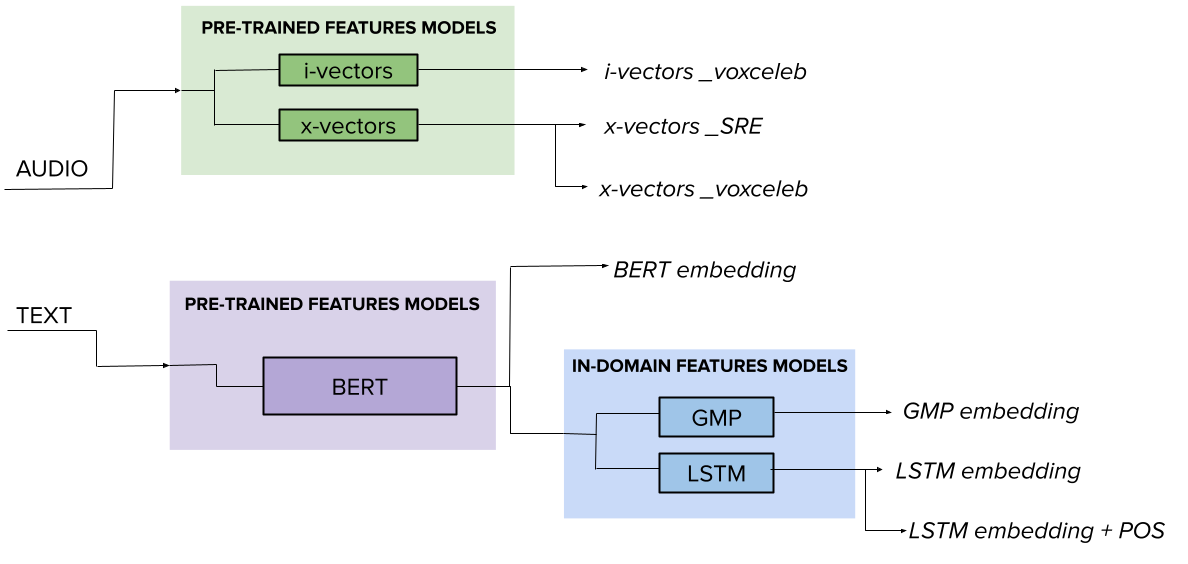
\includegraphics[scale=0.35]{imgs/ADReSS.png}  
  \caption{Overview of the multimodal system based on embeddding appraoches}
  \label{fig:adress_overview}
  \end{center}
\end{figure}
Our multi-modal framework, illustrated in Figure \ref{fig:adress_overview}, is based on the independent generation of acoustic and textual feature embeddings. Subsequently, we conduct an early fusion of the output of the two systems to create a singular feature vector encapsulating a condensed representation of both speech and language characteristics. The final classification is carried out using an SVM classifier with a linear kernel. Further details on the two systems are provided in the subsequent sections.
\subsubsection{Acoustics modality}
The acoustic system incorporates i-vectors and x-vectors. Taking into consideration the small size of the ADReSS dataset, we preferred to exploit already existing pre-trained models to produce our acoustic feature embeddings, rather than training them using in-domain challenge data. For the x-vectors framework, both the SRE and Voxceleb models were employed. The SRE model was primarily trained on telephone and microphone speech using data from the Switchboard corpus, Mixer 6, and NIST SREs \cite{snyder2018x}. The Voxceleb model was trained on augmented VoxCeleb 1 and VoxCeleb 2 datasets, encompassing speech from speakers with diverse ethnicities, accents, professions, and ages \cite{snyder2018x,nagrani17_interspeech}. This dataset was also used to build the i-vectors pre-trained model.

Inputs to these pre-trained models included 23 and 30-dimensional MFCCs extracted with Kaldi \cite{kaldi} and non-speech frames were filtered out using VAD. For x-vectors, a 512-dimensional embedding was extracted, while i-vectors, based on GMM-UBM, with a 400-dimension.
\subsubsection{Linguistic modality}
We pursued two distinct methods to obtain textual feature embeddings. Firstly, we explored training deep architectures on the relatively small corpus with dimension like the one use in this challenge. Then, we compare this approach with a less data-intensive method based extracting sentence embeddings using a pre-trained model. Both strategies use contextual word embeddings as input but produced different types of learned representations as output. To integrate information from linguistic and acoustic systems, trained architectures were employed to extract linguistic features before the final classification layer, resulting in a single 768-dimensional feature vector for an entire description. In contrast, the sentence embedding approach yielded a 768-dimensional vector for each sentence in a description.

For both approaches, the initial pipeline step involved normalising the data in the ADReSS dataset. Clean transcriptions were encoded into 768-dimensional context embedding vectors using a pre-trained English BERT model with 12 layers and 768 hidden units. The first system, derived from the ComParE2020 Elderly Challenge baseline \cite{schuller2020interspeech}, involved training three neural models on top of contextual word embeddings: (i) a Global Maximum pooling, (ii) a bidirectional LSTM (biLSTM) with an attention module, and (iii) the second model augmented with part-of-speech (POS) embeddings. The loss was evaluated during training on the development set.

The second system, do not require additional training phase, as representations are extracted from a pre-trained model to directly characterise linguistic deficits in AD. Contextual word embeddings obtained for each word were used to compute fixed-size embedding vectors for each sentence by averaging the second to twelfth hidden layers of each word.
\subsection{Results}
%In this end, speech signals are encoded into \textit{x-vector} using pre-trained models. For textual input, contextual embedding vectors are first extracted using an English Bert model \cite{Bert} and then used to feed a bidirectional recurrent neural network with attention. This multi-model system, based on the combination of linguistic and acoustic information, attained a classification accuracy of 81.25\%. Results have shown the importance of linguistic features in the classification of Alzheimer’s disease, which outperforms the acoustic ones in terms of accuracy.
\begin{table}[t]
  \begin{center}
  \begin{tabular}{lcccc}
  \hline
  & \multicolumn{1}{l}{\textbf{Accuracy}} & \multicolumn{1}{l}{\textbf{Precision}} & \multicolumn{1}{l}{\textbf{Recall}} & \multicolumn{1}{l}{\textbf{F1 Score}} \\
  \hline
  x-vectors\_Vox           & 0.6818                               & 0.6834                                & 0.6919                             & 0.6812                               \\
  x-vectors\_SRE              & \textbf{0.7273}                               & \textbf{0.7273}                                & \textbf{0.7273}                             & \textbf{0.7273}                               \\
  i-vectors\_Vox          & 0.6818                               & 0.7292                                & 0.6818                             & 0.6645                               \\
  i-vectors\_Vox\_x-vectors\_Vox & 0.7273                               & 0.7273                                & 0.7273                             & 0.7273                               \\
  i-vectors\_Vox\_x-vectors\_SRE      & 0.7273                               & 0.7351                                & 0.7273                             & 0.7250                                \\
  \hline
  \end{tabular}
  \caption{Results of different acoustic approaches on the development set}
  \label{tab:adress_acoustics}    
\end{center}
\end{table}

The results obtained using the different acoustic feature embeddings are summarised in Table \ref{tab:adress_acoustics}. Different independent models were explored, and an early fusion of the best acoustic results was performed. The x-vectors Voxceleb model generally achieved lower classification accuracy; however, when combining i-vectors and x-vectors extracted from this model, the fused accuracy was comparable to x-vectors trained on the SRE corpus, representing the best result on the development set. These outcomes are slightly lower than those reported in similar works in the literature \cite{warnita18_interspeech,zargarbashi2019multi}. However, our approach, distinct from these previous studies as we uses a smaller dataset and do not rely on DNN training. To validate these results on the test set, we select the acoustic feature embeddings extracted from the pre-trained x-vectors SRE model for evaluation.
\begin{table}[t]
  \begin{tabular}{lcccc}
  \hline
& \multicolumn{1}{l}{\textbf{Accuracy}} & \multicolumn{1}{l}{\textbf{Precision}} & \multicolumn{1}{l}{\textbf{Recall}} & \multicolumn{1}{l}{\textbf{F1 Score}} \\ \hline
  Global Max Pool. & 0.7727                               & 0.7947                                & 0.7728                             & 0.7684                               \\
  LSTM-RNNs        & 0.8182                               & 0.8182                                & 0.8182                             & 0.8182                               \\
  LSTM-RNNs Pos    & 0.8636                               & 0.8667                                & 0.8637                             & 0.8634                               \\
  GMax/LSTM-RNNs/LSTM-RNNs-Pos                   & \textbf{0.9091}                               & \textbf{0.9091}                                & \textbf{0.9091}                             & \textbf{0.9091}  \\  
  %\textit{\textbf{Sentence emb.}  }                  & 0.6930                               & 0.6864                                & 0.6903                             & 0.6873  \\
  \textit{\textbf{Sentence emb. - maj. vote}}                    & 0.7727                               &0.7947                & 0.7728                           & 0.7684
  \\ \hline
  \end{tabular}
  \caption{Results of different linguistic approaches on the development set}
  \label{tab:res_dev_ling}
  \end{table}

  The results obtained with our various linguistic systems are shown in Table \ref{tab:res_dev_ling}, presenting the performance for features trained with three neural models, their fusion, and the sentence embeddings approach. For the sentence embeddings approach, the accuracy use a majority voting strategy over the entire description. Our best classification result attained an accuracy of 90.91\% on the development set using the fusion of the linguistic features sets generated by the three neural models. Comparing this result with the one obtained by sentence embeddings, we acknowledge that neural models outperform simpler strategies even with constrained training data. This was somehow surprising and in contradiction with similar experiments performed with the acoustic system. We hypothesise that the large amount of contextual information provided by the Bert model is helpful in overcoming the limited size of the ADReSS dataset. Nevertheless, we suspect that the high accuracy attained with neural models may be too optimistic, due to the fact of having used the development set both for testing and evaluating the model’s loss. Thus, in spite of their lower outcome, the sentence embeddings approach is selected as one of the systems to be evaluated on the test set. In fact, on the one hand, we think that they may represent a more reliable system, since do not require additional training. On the other hand, we also observe that they achieve higher classification scores, when compared with a similar approach based on GloVe embeddings [38], thus corroborating our decision.

  For a comprehensive evaluation of speech and language impairments in AD, we performed an early fusion of the best results from both the acoustic and linguistic systems. This involved merging x-vectors with linguistic feature sets from three neural models. However, results on the development set using this extended feature set did not yield additional improvements. Despite this, we selected the combined system as our primary choice for evaluation.

  \begin{table}[t]
    \begin{center}
    \begin{tabular}{llcccc}
    \hline
     & \textbf{Class} & \multicolumn{1}{l}{\textbf{Accuracy}} & \multicolumn{1}{l}{\textbf{Precision}} & \multicolumn{1}{l}{\textbf{Recall}} & \multicolumn{1}{l}{\textbf{F1 Score}} \\ 
                                         \hline
    Fusion of system   & AD             & \multirow{2}{*}{\textbf{0.8125}}                     & 0.9412                                 & 0.6667                              & 0.7805                                \\
   & non-AD         &                                       & 0.7419                                 & 0.9583                              & 0.8364                                \\
    %                                     & Avg.           & \textbf{0.8125}                       & \textbf{0.8415}                        & \textbf{0.8125}                     & \textbf{0.8085}                       \\
    Sentence embedding & AD             &  \multirow{2}{*}{\textbf{0.7292}}                                    & 0.8235                                 & 0.5833                              & 0.6829                                \\
     & non-AD         & \multicolumn{1}{l}{}                  & 0.6774                                 & 0.8750                              & 0.7636                                \\
    %                                     & Avg.           & 0.7292                                & 0.7505                                 & 0.7292                              & 0.7233                                \\
    x-vectors\_SRE     & AD             & \multirow{2}{*}{\textbf{0.5417}}                                      & 0.5417                                 & 0.5417                              & 0.5417                                \\
    & non-AD         & \multicolumn{1}{l}{}                  & 0.5417                                 & 0.5417                              & 0.5417                                \\ \hline
    %                                     & Avg.           & 0.5417                                & 0.5417                                 & 0.5417                              & 0.5417    \\ \hline
    \end{tabular}
    \caption{Results of different acoustic and linguistic approaches on the test set}
    \label{tab:adress_test}  
  \end{center}
    \end{table}


  For the evaluation, three systems were submitted: (i) a fusion of the best results from linguistic and acoustic systems, (ii) sentence embeddings, and (iii) the best acoustic system. Results on the test set, presented in Table \ref{tab:adress_test}, showed a consistent drop in performance compared to the development set, even for systems not requiring a training phase. The first system achieved the best result with an accuracy of 81.25\%, indicating the capability of deep architectures with contextual word embeddings to overcome dataset limitations. The acoustic system alone yielded the lowest accuracy at 54.17\%, suggesting room for improvement in adapting acoustic pre-trained models, for example, to better model elderly speech characteristics.



\section{Transfer Learning-Based Cough Representations for Automatic Detection of COVID-19}
\subsection{Introduction}
Finally, we further extend the idea of using pre-trained representation to automatically detect COVID-19 from cough recordings. Indeed, the COVID-19 respiratory disease was declared a pandemic by the World Health Organisation on March 2020, with profound personal, societal, and economic consequences. Clinical diagnosis primarily relies on RT-PCR and antigen tests, but these methods have drawbacks such as significant costs, intrusive sample collections, and delays in diagnosis due to laboratory saturation. To address these challenges, there is a growing interest in developing reliable, cost-effective, immediate, and user-friendly tools to optimise screening campaigns for health care operators, institutions, and companies.

In our work \cite{SoleraUrea2021TransferLC}, we contributed to the ComParE 2021 COVID-19 Cough Sub-challenge \cite{schuller21_interspeech}. Firstly, we employ transfer learning to develop COVID-19 classification subsystems using deep cough representation extractors, including TDNN-F and CNN embeddings, as well as PASE+ features. Secondly, we integrate individual decisions from the three experts into a calibrated decision-level fusion system. This ensemble of expert subsystems, relying on cough representations, aims to generate well-calibrated log-likelihood scores across various operating points. The resulting output can be readily interpreted by human experts and seamlessly incorporated into the decision-making process.

Current research on the automatic detection of COVID-19 from speech or respiratory sounds builds on prior studies demonstrating the distinct effects of various respiratory diseases on these sounds. This approach has proven effective in detecting pertussis, asthma, pneumonia, tuberculosis, among others \cite{pramono2016cough}. While conclusive evidence is still pending for COVID-19, preliminary findings suggest specific signatures of COVID-19 in coughs and speech that could potentially enable detection even in apparently asymptomatic individuals and differentiate it from other common respiratory illnesses. Given the limited availability of labeled COVID-19 data, many approaches rely on transfer learning, data augmentation, and class balancing techniques.

The majority of previous work in this domain relies on CNNs. For instance, a pre-trained VGGish model \cite{Hershey2017}is employed as a generic audio feature extractor in \cite{Chloe2020}. Other works fine-tune CNNs initially trained for cough detection for the purpose of COVID-19 detection \cite{Bagad2020,Imran2020}. Ensemble models incorporating both DNNs and CNNs, directly trained from scratch for COVID-19 detection, have also been proposed \cite{Chaudhari2021}. Additionally, certain studies  \cite{Han2021} leverage information about self-reported symptoms, encoding them as one-hot vectors and combining them either at the feature- or decision-levels with traditional speech features.

\subsection{Corpora}
In this work, we used two datasets: the COVID-19 COUGH (C19C) corpus, provided in the ComParE 2021 COVID-19 Cough Sub-Challenge \cite{Chloe2020,Han2021} for evaluation, and the COUGHVID corpus \cite{Orlandic2020}, employed for training and fine-tuning transfer learning-based cough representation extractors. Silence segments were eliminated from both datasets.

The COVID-19 COUGH (C19C) corpus is a subset of the Cambridge COVID-19 Sound database \cite{Chloe2020,Han2021}, consisting of 725 cough recordings from 397 participants with self-reported COVID-19 status labels (positive/negative). The corpus is distributed into train (71 positives/215 negatives), development (48 positives/183 negatives), and a blind test set (208 samples) with gender-balanced subsets. 

In our preliminary analysis, it was observed that some files had a reduced bandwidth of 4 kHz, potentially corresponding to samples originally recorded at 8 kHz. Namely, 13, 8 and 8 narrow-band files were detected in the train, development and test subsets, respectively. This condition certainly reflects the reality of many real-world applications. However, we noticed that all the narrow-band recordings in the train and development subsets correspond to the COVID-19 positive class To address this, a second version of the dataset, denoted as ``$\text{C19C}_{fullband}$", was created by removing narrow-band recordings from the original train and development subsets. This resulted in 273 samples in the train subset (58 positives/215 negatives) and 223 in the development subset (40 positives/183 negatives), while the test subset remained unchanged for consistent challenge evaluation conditions.

The COUGHVID corpus \cite{Orlandic2020} is a publicly open dataset consisting of non-curated recordings performed using lossy codification. The dataset includes a variety of conditions such as sampling rate, bandwidth, number of channels, and quality. Volunteers recorded their coughs and reported their COVID-19 status (positive/symptomatic/healthy), age, gender, and medical condition.
The dataset comprises 27,550 recordings, with 15,125 classified as coughs by an automatic cough detector. Of these, 10,763 have self-provided gender and COVID-19 status annotations, including 680 COVID-19 positives (395 male/285 female), 8,270 healthy (5,632 male/2,638 female), and 1,813 symptomatic (1,114 male/699 female). Additionally, a small fraction of the dataset was annotated by expert pulmonologists with information on various aspects, such as type of cough, presence of audible symptoms, diagnosis, and severity.

\subsection{Proposed system}

\subsubsection{TDNN-F embedddings}
X-vector embeddings are currently regarded as state-of-the-art speaker representations, surpassing other proposed representations like d-vectors and i-vectors. Motivated by the results of the two previous works mentioned in this annex, this study explores the applicability of x-vector-like embeddings to coughs, aiming to encode relevant information about the cough signal for medical insights.
The X-vector extractor is implemented using TDNN-F as proposed for speaker recognition in \cite{villalbaSRE182020}.  Cough embeddings are 128-dimensional vectors obtained at the output of the final dense layer. The network undergoes two-stage training: initially an age estimation and gender classification using a subset of the COUGHVID dataset was performed, and subsequently fine-tuning with expert-annotated data for tasks closely related to COVID-19 classification. These tasks include cough type, presence of dyspnea, presence of wheezing, diagnosis, and severity. The reason behind this fine-tuning step is the fact that these tasks are much closer to COVID-19 classification than age and gender. Input features consist of 30 MFCCs computed every 10 ms from 25 ms-length frames, following the egs/voxceleb/v2 Kaldi recipe \cite{kaldi}.

\subsubsection{CNN embedddings}
CNN-based approaches for COVID-19 detection suffer from some limitations such as the use of CNNs as generic audio feature extractors without task-specific tuning or relying on relatively small datasets for training. In contrast, our work addresses these limitations by leveraging transfer knowledge from the VGGish model, originally trained on a vast corpus for audio classification, and subsequently fine-tuning it for COVID-19 detection using the COUGHVID dataset.

The VGGish model \cite{Hershey2017},  is an adaptation of the VGG network \cite{Simonyan2015} for audio classification. It consists of four blocks with convolutional and pooling layers, followed by fully-connected layers and an output layer. In this work, a simplified version of the model is used and was pre-trained using 5.4 million hours from YouTube data. For our experiments, we used two different settings. In the first setting, the model serves as a pre-trained generic feature extractor with weights directly loaded from the original model. In the second setting, the model is fine-tuned for COVID-19 detection using a balanced subset of the COUGHVID dataset. The input to the VGGish network is log Mel-spectrogram features computed every 0.24 s from 0.96 s-length segments amd the resulting embeddings are 256-dimensional vectors.

When fine-tuning, layers 9 and 10 are included to facilitate training with limited data, with their weights initialized randomly. The entire CNN is fine-tuned for 150 epochs using cross-entropy loss, the Adam optimizer with a learning rate of $10^{-5}$, and a batch size of 64. The fine-tuning is conducted on a balanced subset of the COUGHVID dataset, consisting of 680 positive and 680 negative cough recordings, with 80\% used for training and 20\% for development.

\subsubsection{PASE+ embedddings}
The study incorporates the problem-agnostic speech encoder model, PASE+ \cite{Pascual2019,Ravanelli2020}, g where targets are learned directly from the
signal. PASE+ features are derived from a shared encoder with a SincNet-based layer \cite{Sincnet}, seven convolutional blocks, and a Quasi-RNN layer. The encoder output is connected to twelve workers, each designed for specific tasks like reconstruction of waveform, log power spectrum (LPC), MFCCs, prosody, filter banks (fbanks), gammatone, and binary discrimination tasks. Two PASE+ extractors were used: one pre-trained on Librispeech and another trained from scratch on COUGHVID data. Both are trained for 150 epochs, creating 256-dimensional feature vectors for each frame every 10 ms.
\subsubsection{COVID-19 condition classification}
The study employs transfer learning to address the limited COVID-19 data for training. Three SVMswe used on TDNN-F embeddings, CNN embeddings, and PASE+ features, respectively, for expert decisions. TDNN-F embeddings are directly input to the SVM. CNN-based embeddings are derived from cough segments and subjected to majority voting for the final decision. PASE+ features are averaged across the sequence and fed to the SVM classifier. The SVMs are trained on both the C19C and $\text{C19C}_{fullband}$ datasets, exploring various kernels, data normalisations, and class balancing methods. Hyperparameters are optimised through grid-search on development subsets, and linear logistic regression is applied to combine system decisions with scaling factors. The regression approximates log-likelihood ratios, thus, a theoretically determined decision threshold can be used for making hard decisions.
\subsection{Results}
\begin{table}[]
  \begin{center}
    
  \begin{tabular}{c|c|c|c}
  \hline
  \multicolumn{1}{c|}{\textbf{System}} & $dev$ & $dev_{fullband}$ & $test$ \\ \hline
  \multicolumn{4}{c}{\textbf{ComParE 2021 CCS Sub-challenge Baseline}} \\ \hline
  {\scriptsize OPEN}SMILE & 61.4 & 53.0 & 65.5 \\
  {\scriptsize OPEN}XBOW\textsubscript{2000} & 64.7 & 56.5 & 72.9 \\
  D{\scriptsize EEP}S{\scriptsize PECTRUM}+SVM & 63.3 & 57.3 & 64.1 \\
  {\scriptsize AU}DEEP\textsubscript{-60 dB} & 67.6 & 57.3 & 67.6 \\
  End2You & 61.8 & - & 64.7 \\
  Fusion of Best & - & - & 73.9 \\ \hline
  
  \multicolumn{4}{c}{\textbf{TDNN-F Embeddings}} \\ \hline
  Trained COUGHVID\textsubscript{Step1} & 68.8 & 63.6 & - \\
  Fine-tuned COUGHVID\textsubscript{Step2} & 68.1 & 62.3 & - \\ \hline
  
  \multicolumn{4}{c}{\textbf{CNN Embeddings}} \\ \hline
  Pre-trained YouTube & 66.9 & 62.4 & - \\
  Fine-tuned COUGHVID & 71.2\textsuperscript{+} & 65.6 & 62.3\textsuperscript{+} \\ \hline
  
  \multicolumn{4}{c}{\textbf{PASE+ Features}} \\ \hline
  Trained Librispeech & 63.1 & 61.7 & -  \\
  Trained COUGHVID & 67.4 & \textbf{66.8}\textsuperscript{+} & 64.1\textsuperscript{+} \\ \hline
  
  \multicolumn{4}{c}{\textbf{Calibrated Fusion}} \\ \hline
  Fusion of experts & \textbf{72.3}\textsuperscript{+} & 66.1 & 69.3\textsuperscript{+} \\ \hline
  \end{tabular}
  \caption{Performance results (unweighted average recall-UAR) on the COVID-19 COUGH (C19C) corpus}
  \label{tab:res_covid}

\end{center}
  \end{table}

  Table \ref{tab:res_covid} shows the comparison between ComParE 2021 CCS baselines and our proposed system. All systems were separately trained on both the C19C and $\text{C19C}_{fullband}$ subsets, and evaluations were conducted on the corresponding dev and $\text{dev}_{fullband}$ subsets. The reported test results are based on the best individual systems trained on the C19C and $\text{C19C}_{fullband}$ datasets (marked with +), presented in terms of unweighted average recall (UAR).

  The proposal demonstrates competitive performance compared to baseline systems. The TDNN-F x-vector embeddings-based expert, trained initially on gender classification and age regression tasks using COUGHVID data, achieves a UAR of 63.6\% on devfullband. However, fine-tuning in step 2 using a multi-task setting does not significantly enhance cough representations, suggesting potential overfitting for some subtasks with limited data.
  
  The CNN embeddings pre-trained on YouTube videos exhibit reasonable performance, improving to 65.6\% UAR after fine-tuning with COVID-19-specific data. The PASE+ features, trained with COUGHVID data, yield the best performance among the three expert systems, with a development UAR of 66.8\% and a test UAR of 64.1\%. Notably, the PASE+ extractor trained on the larger Librispeech dataset achieves a 5.1\% absolute improvement in UAR when trained with COVID-19-specific data, indicating the significant benefit of such data.
  
  The fusion of the best x-vector (Trained COUGHVIDStep1), CNN (Fine-tuned COUGHVID), and PASE+ (Trained COUGHVID) experts yields a UAR of 72.3\% on development (1.1\% absolute improvement from the best expert) and 69.3\% on test when trained on the C19C datasets. The underperformance on the $\text{C19C}_{fullband}$ subset warrants further analysis but may be attributed to the low number of COVID-19 positive examples.

%We leverage transfer learning to develop a set of COVID-19 classification subsystems based on deep cough representation extractors called experts. Individual decisions of three experts are fed to a calibrated decision-level fusion system. This ensemble of expert subsystems based on cough representations is expected to produce well-calibrated log-likelihood scores over a wide range of operating points. The output can be more easily interpreted by a human expert and incorporated into the decision-making process. Our results show competitive performance compared to hand-crafted features, although they are still far from those required to become a reliable tool to assist COVID-19 screening.

\section{Conclusion and future work}
In the three distinct research works done within the context of this thesis, we employed pre-trained embedding extractors as tools for detecting pathologies. These embeddings can be used in two different way: functioning either directly as feature extractors or undergoing fine-tuning for specific tasks. Our findings in these works present promising results, indicating that embeddings trained on substantial amounts of data may contain valuable health-related information.

We began by exploring the replacement of knowledge-based features with task-agnostic speaker representations in multiple disease detection. Focusing on x-vector embeddings trained with elderly speech data, our experiments with European Portuguese datasets supported the hypothesis that discriminative speaker embeddings, particularly x-vectors, contain relevant information for disease detection that knowledge-based features may fail to represent. Notably, x-vectors proved more suitable than i-vectors for tasks with domain mismatches, such as verbal task mismatches and cross-lingual experiments. Future endeavors include training the x-vector network with augmented and multilingual datasets, extending the approach to other diseases and verbal tasks, and replicating experiments with in-the-wild data collected from online multimedia repositories.

Moving to the context of AD classification, we adopted a multi-modal approach, leveraging automatically learned feature representations. Our investigation covered both acoustic and linguistic, exploring feature embedding vectors from pre-trained models and training deep neural architectures. By combining these approaches, we achieved an accuracy of 90.91\% and 81.25\% on the development and test sets, respectively. Notably, acoustic systems demonstrated a greater need for data to improve predictive ability, especially in the presence of potential ASR errors. Future work may involve analysing the impact of ASR errors, exploring robust acoustic methods tailored to AD speech characteristics, and delving into the implications of atypical speech.

Lastly, our focus shifted to the ComParE 2021 COVID-19 Cough Sub-challenge. Leveraging transfer learning, we developed three expert classifiers: TDNN-F embeddings, CNN embeddings, and PASE+ features. While our results demonstrated competitive performance compared to baseline systems, caution is warranted due to the limited data. To enhance the reliability of COVID-19 screening tools, larger datasets are recommended for better learning of cough representations, coupled with more suitable backend classifiers. Future exploration could includes recurrent neural networks with attention mechanisms to capture temporal dynamics, SSL, multi-task TDNN-F network-based cough embeddings, and assessing the suitability of PASE+ features as an alternative input representation.

Collectively, these contributions showcase the diverse applications of advanced technologies in addressing challenges in health-related tasks using pre-trained representations, ranging from COVID-19 screening through cough analysis to AD classification and beyond, ultimately paving the way for impactful advancements in SLT. 